\documentclass{minimal}
\usepackage{graphicx,color}
\usepackage[utf8]{inputenc}
\usepackage[papersize={420.00bp,315.00bp},text={420.00bp,315.00bp}]{geometry}
\begin{document}
\centering
% Title: gl2ps_renderer figure
% Creator: GL2PS 1.4.2, (C) 1999-2020 C. Geuzaine
% For: Octave
% CreationDate: Mon Dec 12 15:34:17 2022
\setlength{\unitlength}{1pt}
\begin{picture}(0,0)
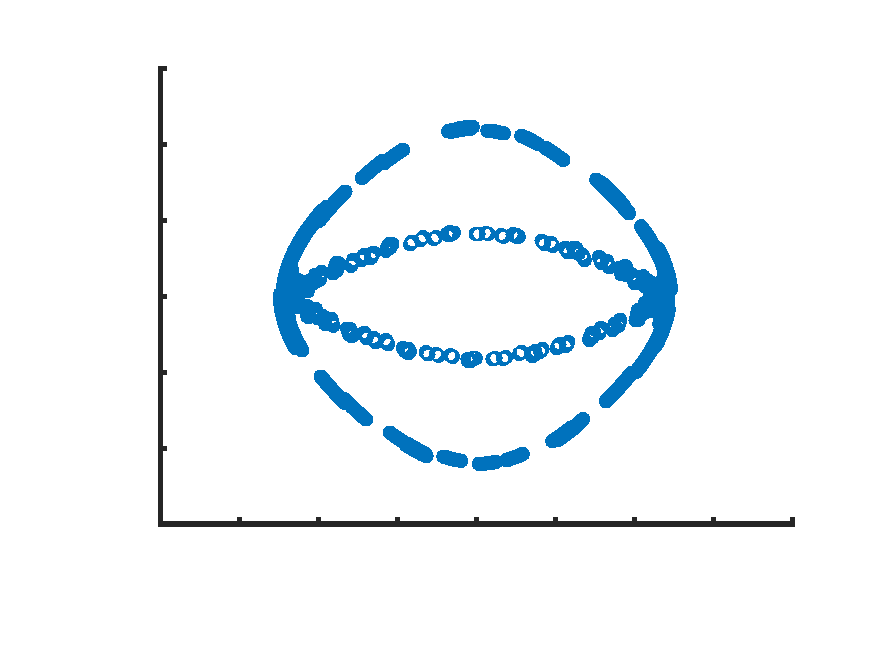
\includegraphics[scale=1]{DoublePoincare-inc}
\end{picture}%
\begin{picture}(420,315)(0,0)
\fontsize{22}{0}\selectfont\put(77.0093,46.8623){\makebox(0,0)[t]{\textcolor[rgb]{0.15,0.15,0.15}{{-0.2}}}}
\fontsize{22}{0}\selectfont\put(114.916,46.8623){\makebox(0,0)[t]{\textcolor[rgb]{0.15,0.15,0.15}{{-0.15}}}}
\fontsize{22}{0}\selectfont\put(152.824,46.8623){\makebox(0,0)[t]{\textcolor[rgb]{0.15,0.15,0.15}{{-0.1}}}}
\fontsize{22}{0}\selectfont\put(190.731,46.8623){\makebox(0,0)[t]{\textcolor[rgb]{0.15,0.15,0.15}{{-0.05}}}}
\fontsize{22}{0}\selectfont\put(228.638,46.8623){\makebox(0,0)[t]{\textcolor[rgb]{0.15,0.15,0.15}{{0}}}}
\fontsize{22}{0}\selectfont\put(266.545,46.8623){\makebox(0,0)[t]{\textcolor[rgb]{0.15,0.15,0.15}{{0.05}}}}
\fontsize{22}{0}\selectfont\put(304.452,46.8623){\makebox(0,0)[t]{\textcolor[rgb]{0.15,0.15,0.15}{{0.1}}}}
\fontsize{22}{0}\selectfont\put(342.359,46.8623){\makebox(0,0)[t]{\textcolor[rgb]{0.15,0.15,0.15}{{0.15}}}}
\fontsize{22}{0}\selectfont\put(380.266,46.8623){\makebox(0,0)[t]{\textcolor[rgb]{0.15,0.15,0.15}{{0.2}}}}
\fontsize{22}{0}\selectfont\put(66,63.3369){\makebox(0,0)[r]{\textcolor[rgb]{0.15,0.15,0.15}{{-1.5}}}}
\fontsize{22}{0}\selectfont\put(66,99.7807){\makebox(0,0)[r]{\textcolor[rgb]{0.15,0.15,0.15}{{-1}}}}
\fontsize{22}{0}\selectfont\put(66,136.225){\makebox(0,0)[r]{\textcolor[rgb]{0.15,0.15,0.15}{{-0.5}}}}
\fontsize{22}{0}\selectfont\put(66,172.668){\makebox(0,0)[r]{\textcolor[rgb]{0.15,0.15,0.15}{{0}}}}
\fontsize{22}{0}\selectfont\put(66,209.112){\makebox(0,0)[r]{\textcolor[rgb]{0.15,0.15,0.15}{{0.5}}}}
\fontsize{22}{0}\selectfont\put(66,245.556){\makebox(0,0)[r]{\textcolor[rgb]{0.15,0.15,0.15}{{1}}}}
\fontsize{22}{0}\selectfont\put(66,282){\makebox(0,0)[r]{\textcolor[rgb]{0.15,0.15,0.15}{{1.5}}}}
\fontsize{24}{0}\selectfont\put(228.638,24.8623){\makebox(0,0)[t]{\textcolor[rgb]{0.15,0.15,0.15}{{$\theta_2/(2 \pi)$}}}}
\fontsize{24}{0}\selectfont\put(24,172.668){\rotatebox{90}{\makebox(0,0)[b]{\textcolor[rgb]{0.15,0.15,0.15}{{$\omega_2$}}}}}
\fontsize{24}{0}\selectfont\put(228.638,292){\makebox(0,0)[b]{\textcolor[rgb]{0,0,0}{{Poincaré Section at $\theta_1 = 0$}}}}
\end{picture}
\end{document}
